\chapter{Descrizione del DS4H Image Alignment Tool}
\label{chap:descriptionoldtool}
\noindent Il capitolo corrente descrive la prima versione del plugin \textit{DS4H Image Alignment}, progetto sviluppato da Stefano Belli nel 2019 come Tesi Magistrale in questo corso di studi.

\subsection{Struttura generale}
\noindent Il plugin ha una interfaccia utente organizzata in finestre modali. Le principali sono:
\begin{itemize}
	\item MainDialog - è la finestra incaricata di mostrare l’immagine corrente. Permette di aggiungere corners per l’allineamento manuale, e da accesso a tutte le altre finestre di dialogo del software.
	\item PreviewDialog - mostra una anteprima delle immagini riportando la lista delle coordinate dei corners già inseriti.
	\item RemoveDialog - permette di rimuovere le immagini precedentemente caricate.
	\item AlignDialog - finestra che mostra il risultato della co-registrazione delle immagini tramite corners, permette di salvare il risultato in file TIFF o di riutilizzare le stesse immagini per un nuovo ciclo di co-registrazione.
\end{itemize}

\noindent Le interazioni con l’utente vengono gestite dalla classe ImageAlignment, allaquale vengono comunicate le operazioni eseguite dalle finestre di dialogo tramite ActionListeners. Le immagini all’interno di \textit{ImageJ} sono incapsulate attraverso la classe ImagePlus, questo garantisce compatibilità con il framework SciJava. Per gestire le immagini viene usata una classe chiamata ImagesManager, che permette di scorrere le immagini caricate da parte dell’utente, reso possibile tramite l’implementazione dell’interfaccia ListIterator.
Le immagini sono racchiuse all’interno di BufferedImage che ne gestisce la visualizzazione; ogni immagine è racchiusa all’interno di una collezione chiamata ImageFile che permette l’estrazione metadati tramite la libreria bio-formats e restituisce il numero di immagini, la dimensione massima, la lista dei corner points registrati tramite ROIManager, etc.
Come si può notare dallo schema in \Cref{fig:9}, ogni istanza di BufferedImage viene generata a richiesta del rispettivo ImageFile per ridurre in maniera efficiente l’utilizzo della memoria.

\begin{figure}[H]
    \centering
    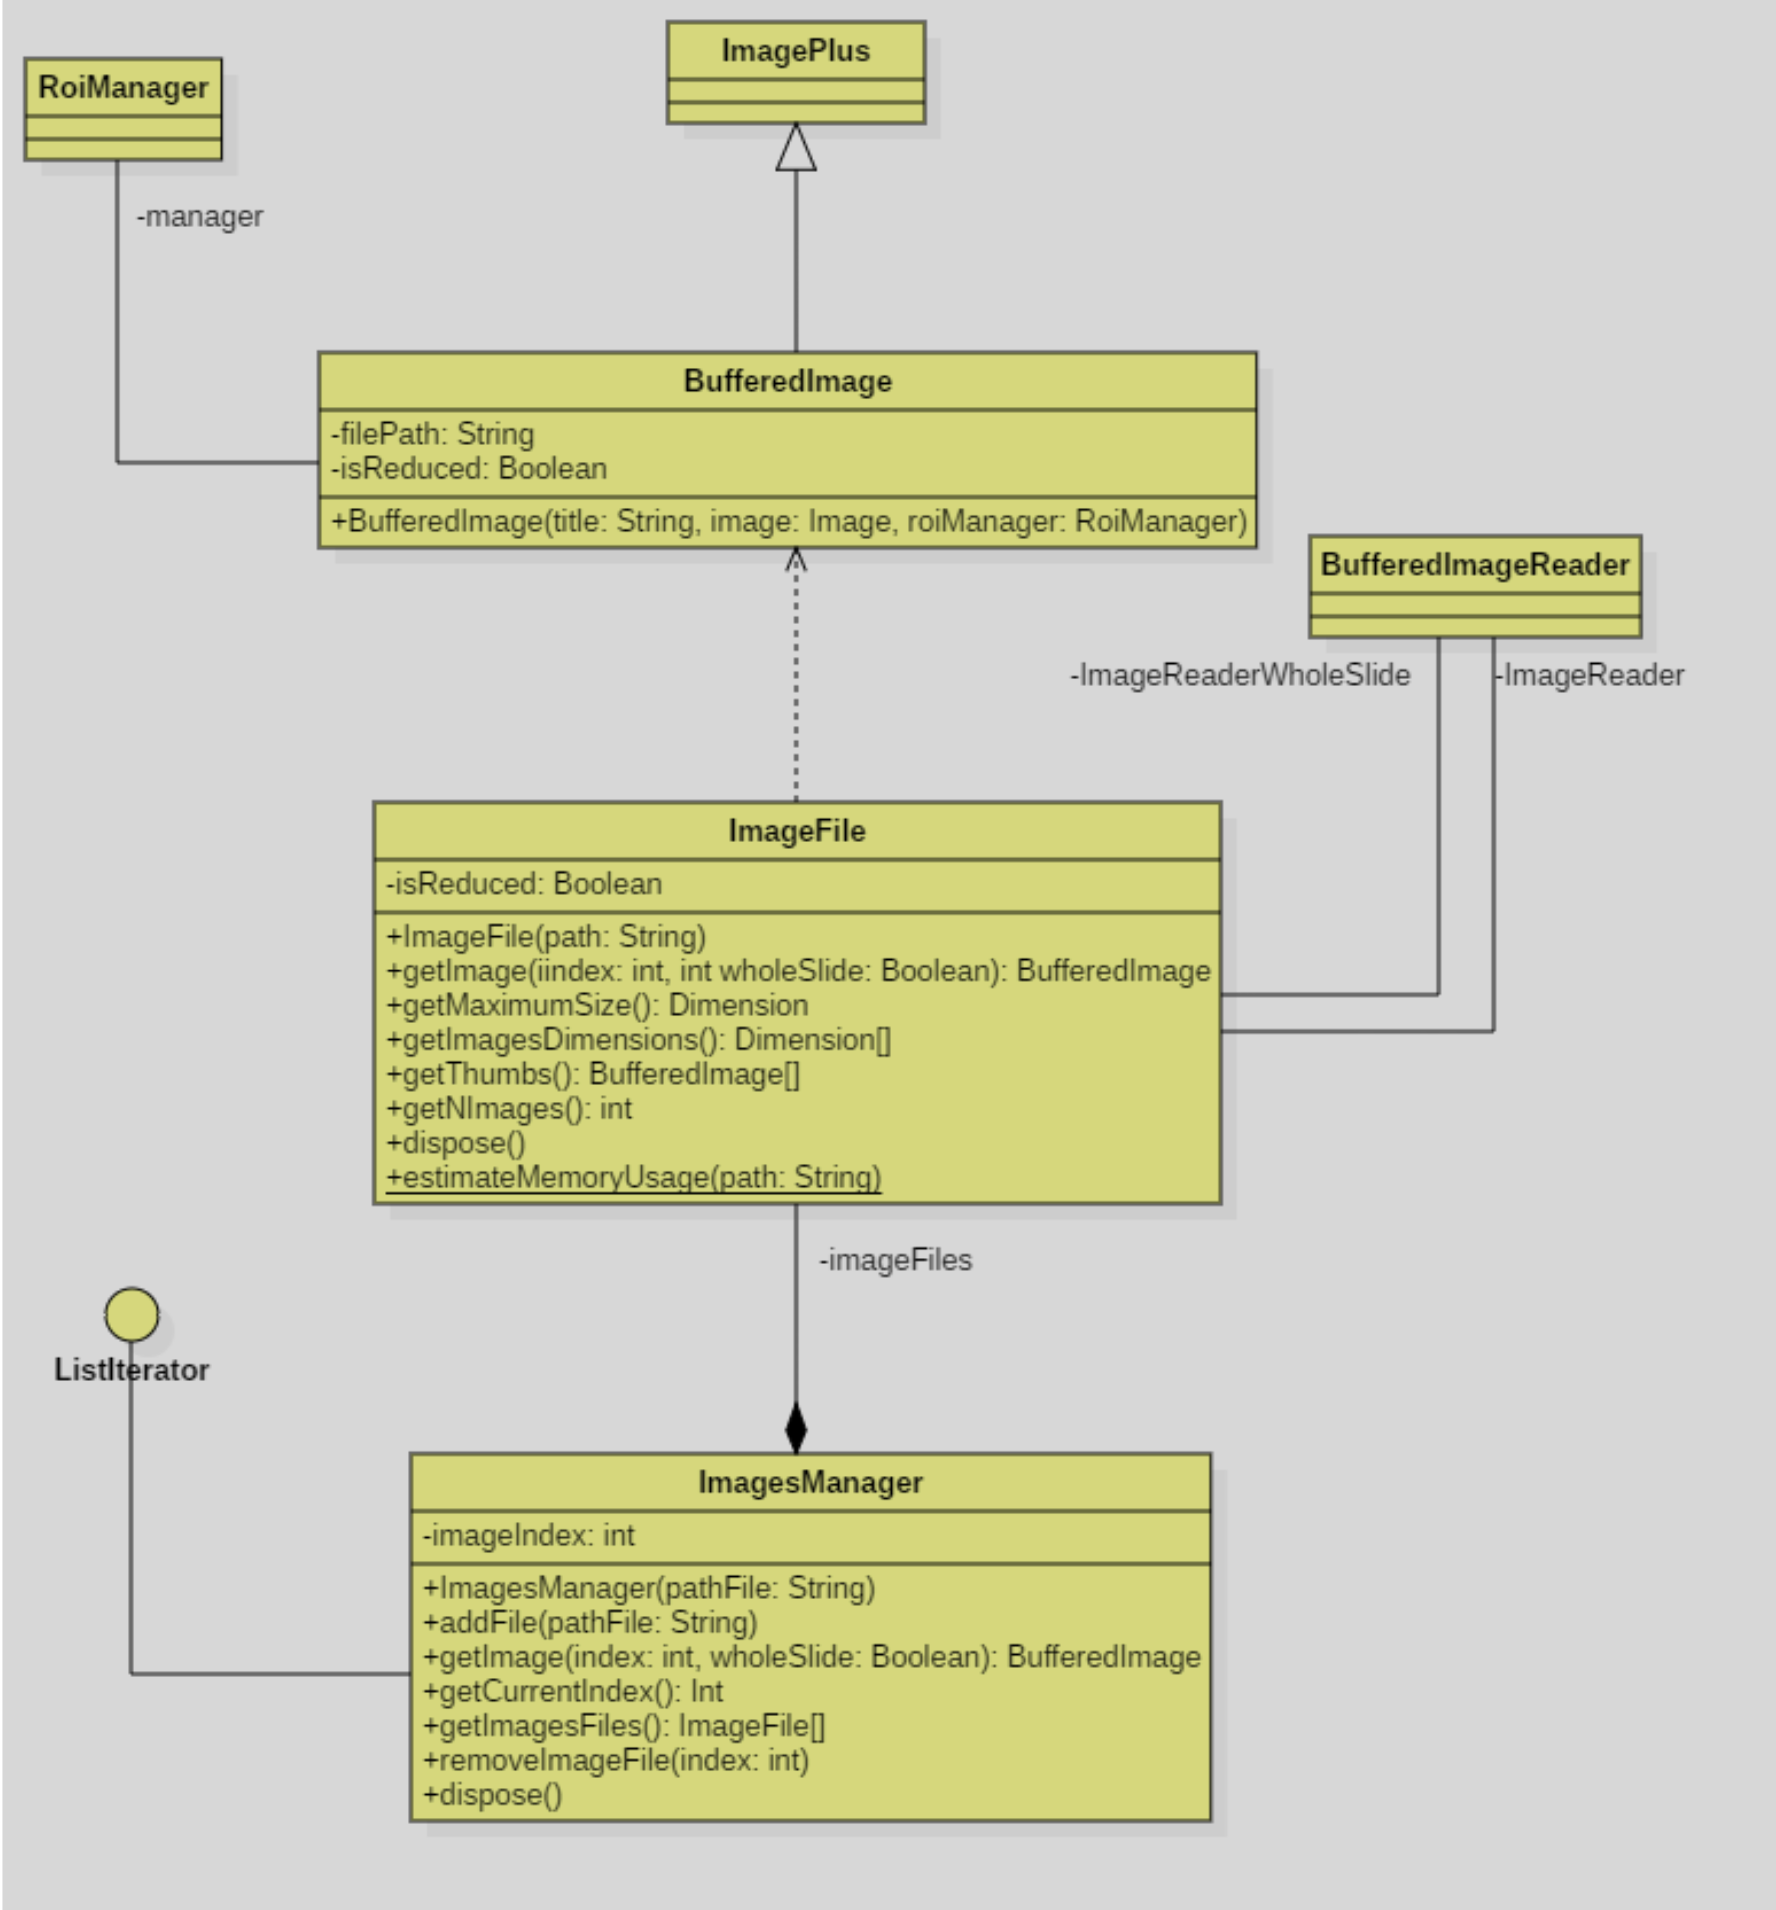
\includegraphics[scale=0.4,keepaspectratio]{SchemaImagePlus.png}
    \caption{Diagramma UML delle classi dati principali di DS4H}
    \label{fig:9}
\end{figure}


\subsection{Modalità d'uso dell'applicazione DS4H}
\noindent Di seguito sono spiegate tutte le funzionalità che il team di sviluppo ha provveduto a rendere disponibili all'utente.
Le schermate presentate in questa sezione provengono da un Macbook Pro M1 Pro.

\subsubsection{Aggiunta Corner Point}
\noindent Basta premere il tasto \textbf{C} all'interno dei limiti dell'immagine corrente, e rispettivamente al punto in cui si è premuto il tasto si mostrera un corner point.
L'esempio in \Cref{fig:10} mostra il risultato dell'operazione, dove si è premuto tre volte, e da cui si può notare l'ordine grazie alla numerazione.
\begin{figure}[H]
    \centering
    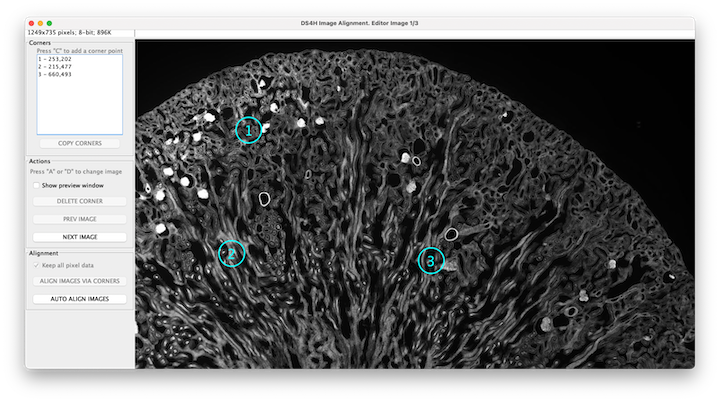
\includegraphics[scale=0.5,keepaspectratio]{windows/aggiunta_corner.png}
    \caption{Schermata principale in cui sono stati aggiunti dei corner points}
    \label{fig:10}
\end{figure}

\subsubsection{Modifica Corner Point}
\noindent Ogni corners point è modificabile nella sua forma trascinandolo tramite cursore come in \Cref{fig:11}.
\begin{figure}[H]
    \centering
    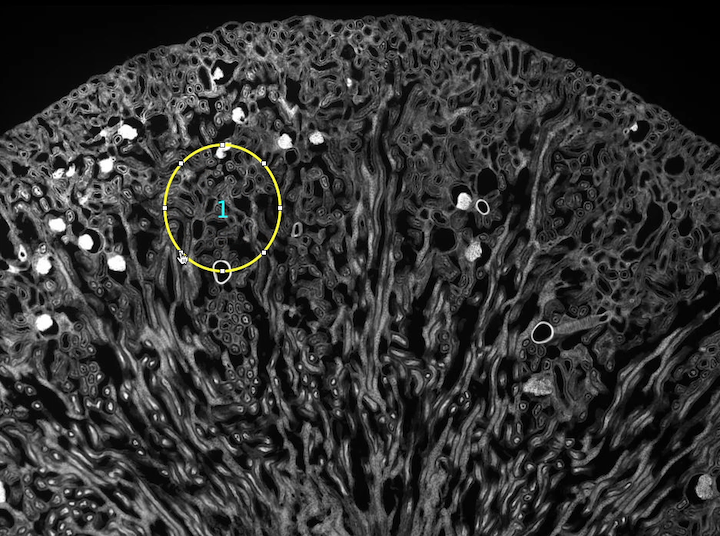
\includegraphics[scale=0.5,keepaspectratio]{windows/modifica_corner.png}
    \caption{Immagine corrente in cui sta venendo modificato un corner}
    \label{fig:11}
\end{figure}

\subsubsection{Rimozione Corner Point}
\noindent Ogni corner point una volta registrato è visibile e selezionabile anche attraverso una lista nella parte sinistra della finestra principale, ed una volta selezionato tramite cursore si può cancellare premendo il bottone in \Cref{fig:12} (``Delete Corner'').

\subsubsection{Cambia Image Corrente}
\noindent I botttoni ``Next Image'' e ``Prev Image'' in \Cref{fig:12} se premuti permettono di navigare tra le immagini importate.

\begin{figure}[H]
    \centering
    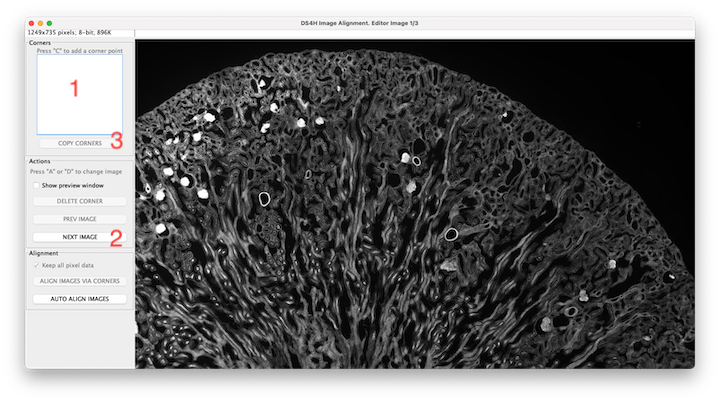
\includegraphics[scale=0.5,keepaspectratio]{windows/schermata_principale.png}
    \caption{Schermata principale i cui numeri definiscono: 1 Rimozione Corner, 2 Cambia Immagine, 3 Copia Corner}
    \label{fig:12}
\end{figure}

\subsubsection{Copia Corner Points}
\noindent Per facilitare l'apposizione dei corners in tutte le immagini l'applicazione è fornita di un bottone apposito visibile in \Cref{fig:12} che se premuto mostra una finestra di dialogo, come quello mostrato in \Cref{fig:13}. Da questa finestra è possibile scegliere l'immagine da cui importare i corner points, e nel caso in cui i corner points importati risultino fuori dai limiti delle immagini il sistema notifica l'utente di ciò, dando la possibilità di cancellare anche dall'immagine sorgente i suddetti punti \Cref{fig:14}.

\begin{figure}[H]
    \centering
    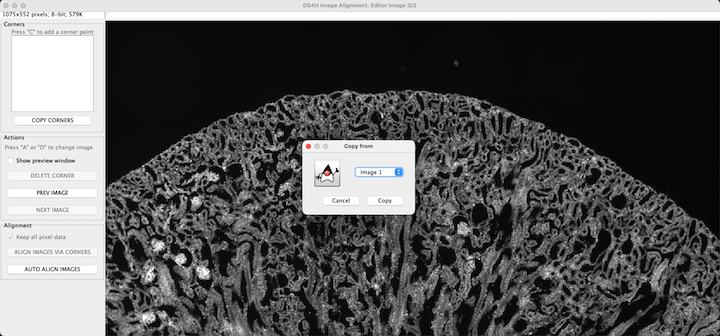
\includegraphics[scale=0.5,keepaspectratio]{windows/copy_corner_from_source.png}
    \caption{Finestra di dialogo da cui si può scegliere l'immagine sorgente per eseguire la copiatura}
    \label{fig:13}
\end{figure}

\begin{figure}[H]
    \centering
    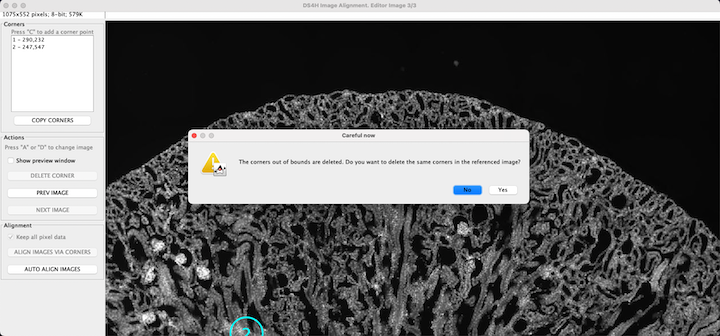
\includegraphics[scale=0.5,keepaspectratio]{windows/copy_corner_warning.png}
    \caption{Finestra di warning che notifica l'utente la presenza di corners fuori dai limiti dell'immagine}
    \label{fig:14}
\end{figure}

\subsubsection{Aggiunge e Rimuove File}
\noindent Dalla finestra principale, accedendo al menu ``File'' si possono eseguire sia l'importazione di una nuova immagine da aggiungere alla presente lista di immagini, sia rimuovere un immagine a scelta.

\begin{figure}[H]
    \centering
    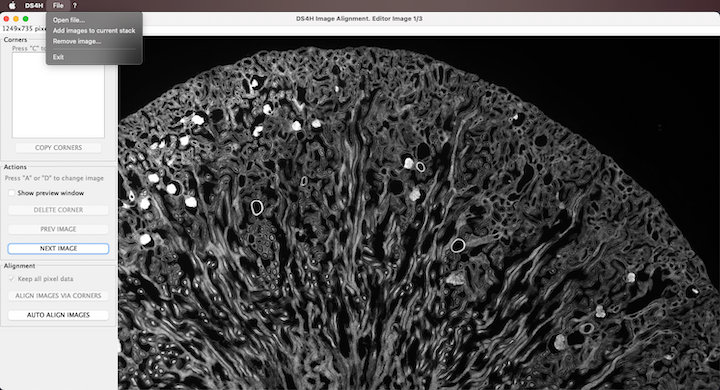
\includegraphics[scale=0.5,keepaspectratio]{windows/menu_principale.png}
    \caption{Schermata principale in cui sono stati aggiunti dei corner points}
    \label{fig:15}
\end{figure}

\subsubsection{Selezione multipla}
\noindent Solo via lista

\subsubsection{Esecuzione Co-registrazione}
\noindent Button + modal scelta
\subsubsection{Salvare Immagine risultante}
\noindent VirtualStack
\subsubsection{Riutilizza Immagine}
\noindent VirtualStack

\subsubsection{Apre Finestra di preview}
\noindent PreviewDialog
\subsubsection{Cmbia immagine di preview}
\noindent PreviewDialog


\subsection{OME Data Model}
\noindent 